\chapter{Produção Científica}
\label{cap:cap3}

Neste Capítulo apresentamos produções científicas em formato de artigos.

Na Sessão~\ref{sec:paper_01}, um artigo publicado que apresenta uma aplicação do \dmc~na análise de dados registrados por um Eletroencefalograma no decorrer de um experimento.

Na Sessão~\ref{sec:paper_02} temos o artigo, em fase de revisão pelos autores, que deve ser submetido em seguida. O artigo trata da implementação de uma ferramenta computacional para facilitar o uso das funções e coeficientes abordados por pesquisadores.

A Sessão~\ref{sec:paper_03} apresenta a ferramenta computacional e explora suas potencialidades.

Ressaltamo que o artigo apresentado no Anexo~\ref{an:a}, foi o primeiro que participei como coautor neste grupo de pesquisa. Ele embasa os trabalhos do artigo apresentado nas Sessões~\ref{sec:paper_01} e \ref{sec:paper_03}, e faz parte da trajetória de investigação sobre os algoritmos que levaram ao artigo apresentado na Sessão~\ref{sec:paper_02}.

\section{Artigo 01: DCCA multi cross-correlation analysis applied on EEG signals to study motor
activity (Real/Imaginary)}\label{sec:paper_01}

\begin{flushright}
    ``That brain of mine is something more\\
    than merely mortal, as time will show.''\\[10px]
    (Ada Lovelace)
\end{flushright}

O primeiro artigo apresentado, \emph{DCCA multi cross-correlation analysis applied on EEG signals to study motor activity (Real/Imaginary)}~\cite{RIBEIRO2025107419}, narra uma pesquisa utilizando o \dmc~na busca de padrões cerebrais, através do estudo das séries temporais oriundas de um experimento (de movimentos reais e imaginários dos membros do corpo) monitorado pelas gravações das ondas do cérebro por um aparelho de eletroencefalograma. O artigo trabalha com o \pdcca com a mesma fonte de dados que o artigo intitulado \emph{Statistical study of the EEG in motor tasks (real and imaginary)}~\cite{Oliveira2023}, utilizando o \pdcca~apresentado no Anexo~\ref{an:a}, e representa um avanço técnico em relação ao anterior.

\begin{figure}[!htb]
    \centering
	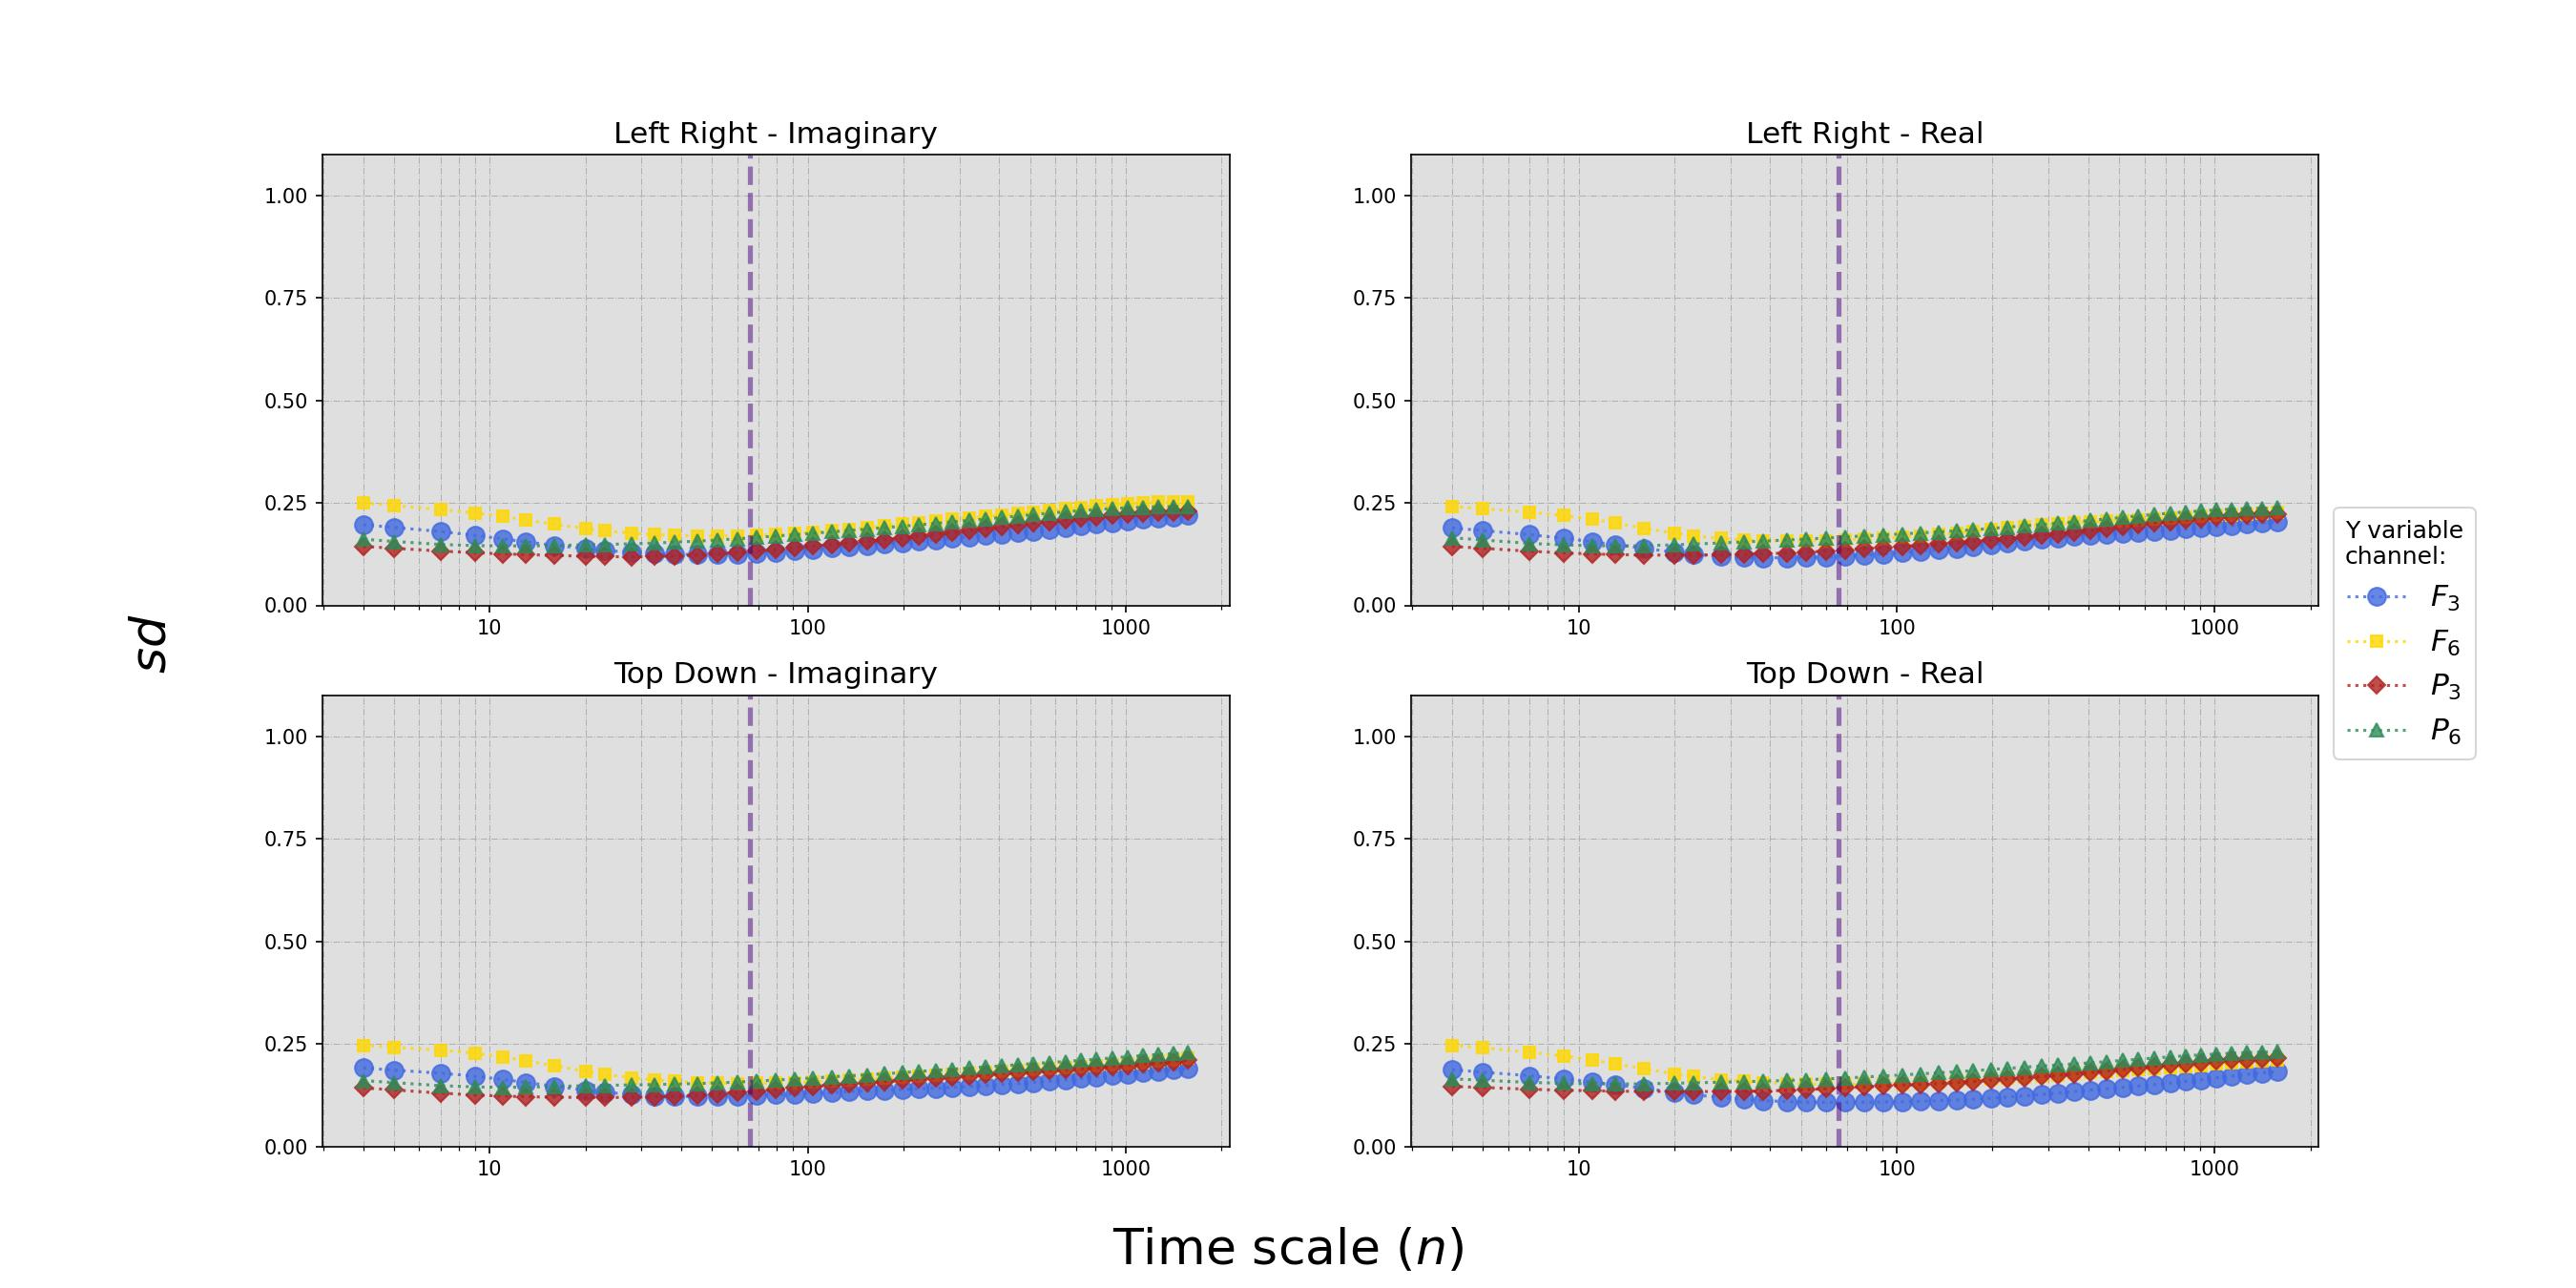
\includegraphics[width=.8\textwidth]{./Figures/art_01/std pop.jpg}
    \captionsetup{justification=centering}
    \caption{Desvio padrão dos valores do \dmc para cada uma das tarefas.\\Fonte: Elaborada pelos autores.}

    \label{fig:a01_sd}
	
\end{figure}

No Artigo de 2023, apenas um subconjunto de 11 indivíduos de universo de 109. Já no artigo de 2025, 108 dos 109 indivíduos foram analisados. Encarando o dilema de, trabalhar com um ambiente de mais alto nível, capaz de manipular o conjunto de dados e visualizar os resultados de foma mais prática e automatizada, com sacrifício do desempenho, ou trabalhar em baixo nível, como maior velocidade de cálculos e menor praticidade para trabalhar, uma solução intermediária foi adotada: os dados foram baixados, carregados, editados e preparados utilizando um ambiante Python, os cálculos foram feitos através de um programa escrito em C e a visualização dos resultados novamente em Python. As chamadas do programa em C foram feitas dentro do código Python, utilizando a biblioteca \emph{subprocess}.

\begin{figure}[!htb]
	\centering
	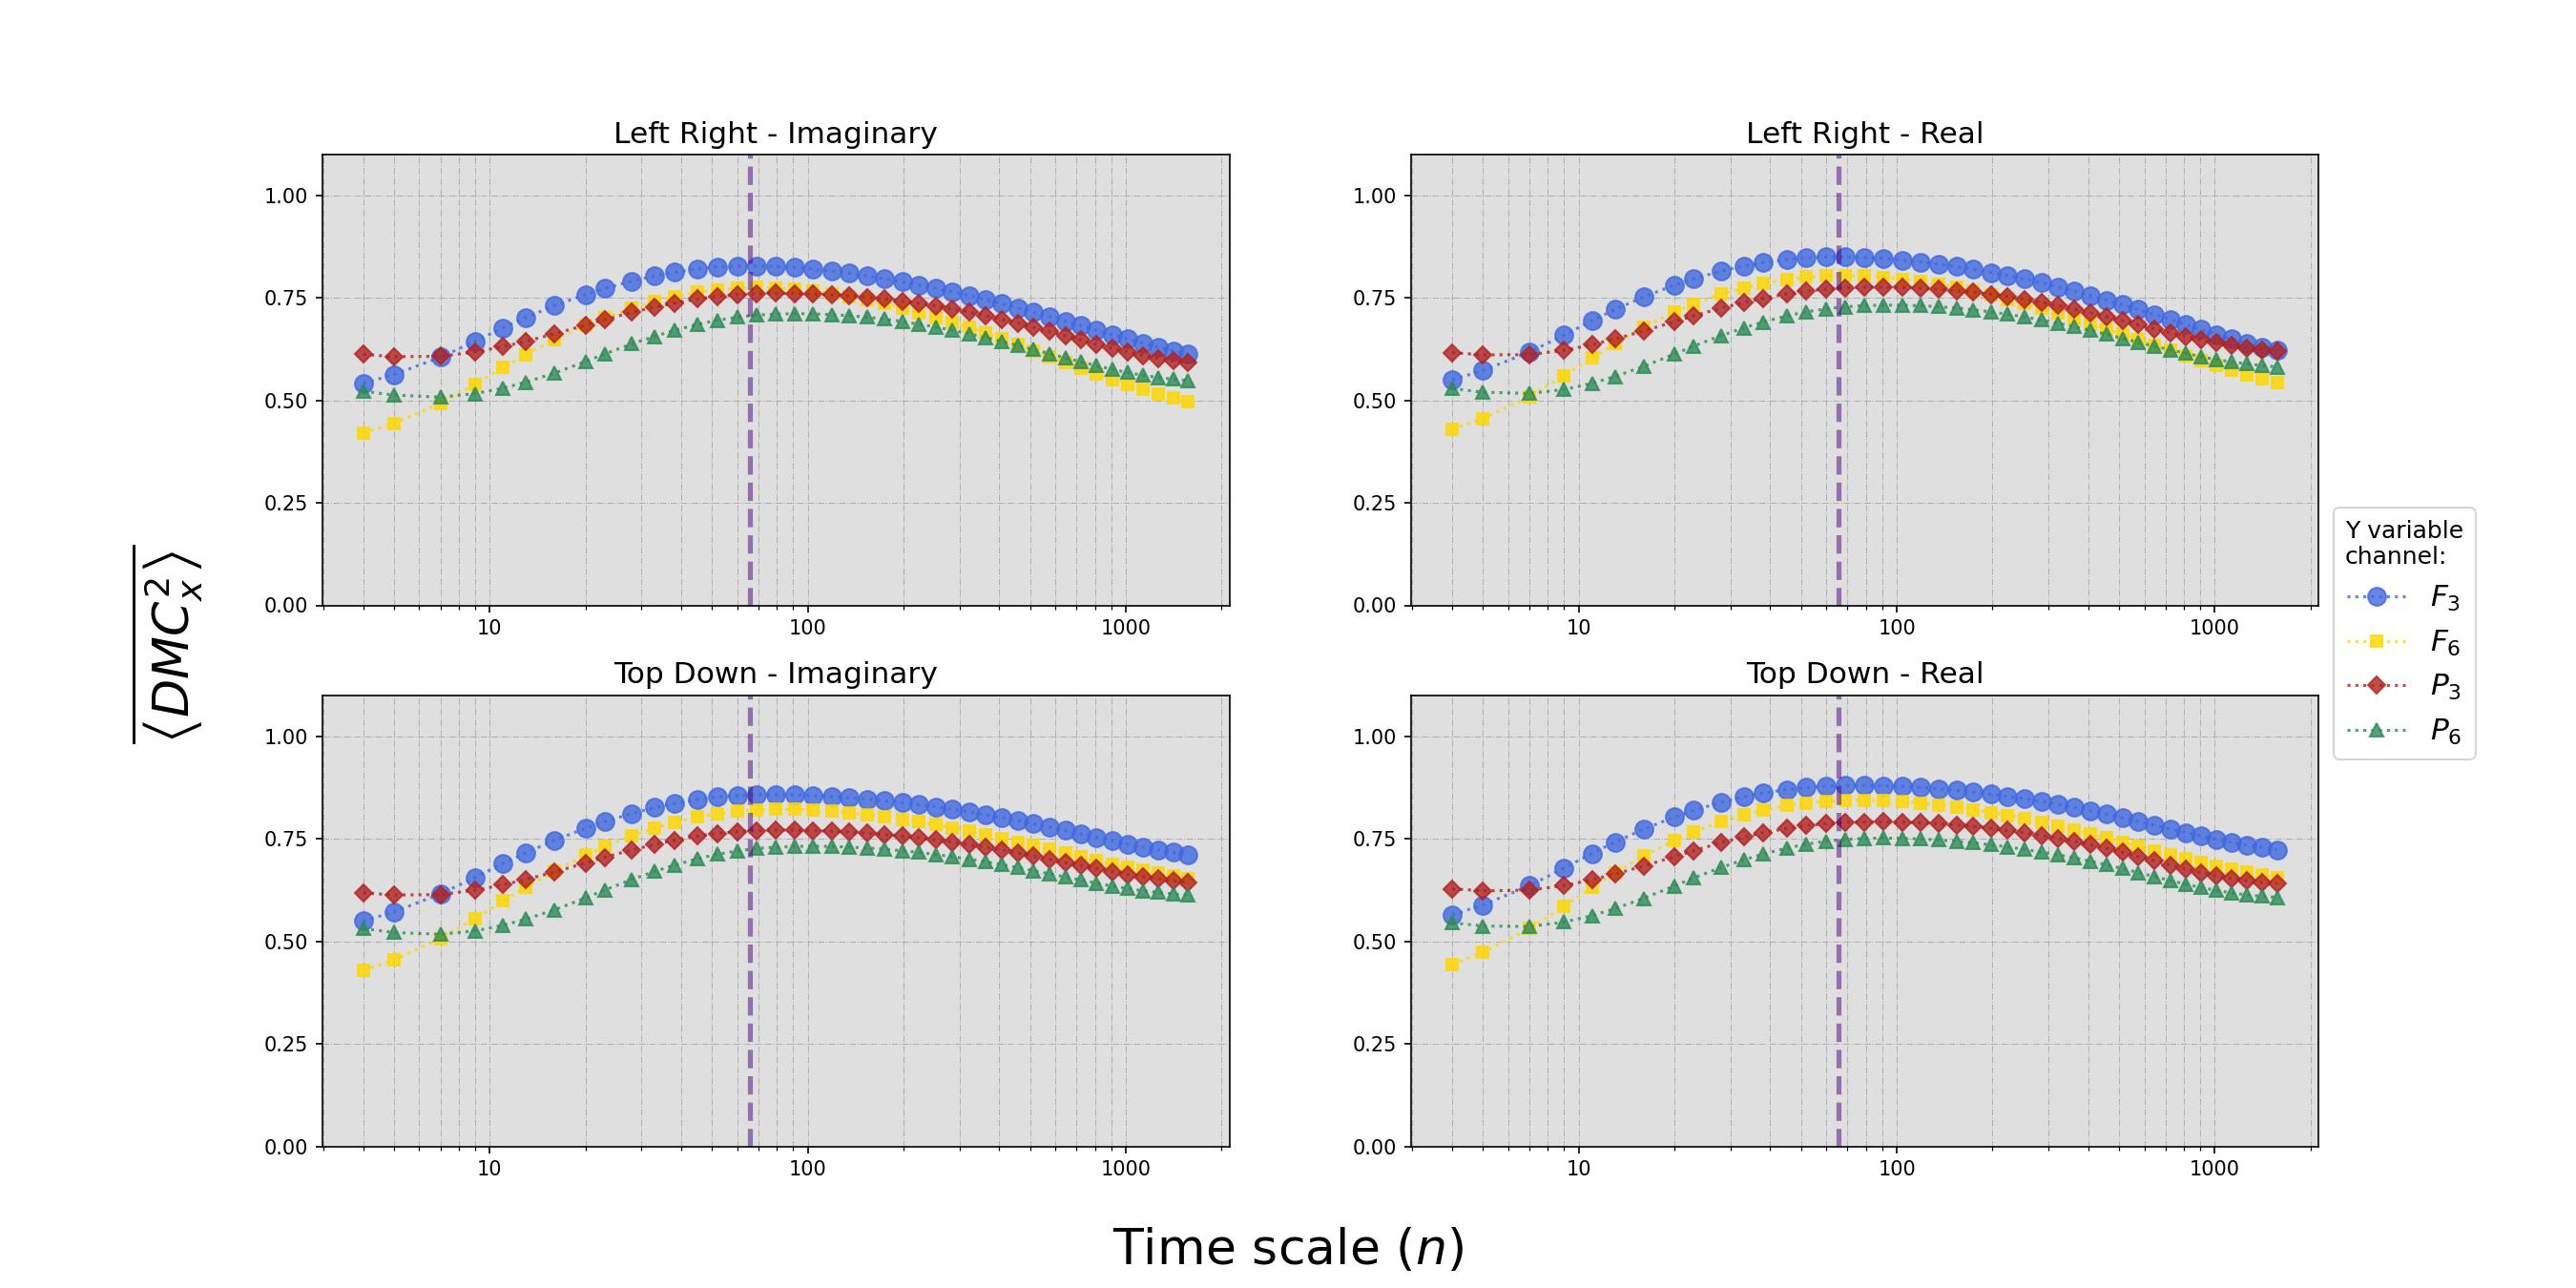
\includegraphics[width=.8\textwidth]{./Figures/art_01/mean.jpg}
    \captionsetup{justification=centering}
    \caption{Médias dos valores do \dmc para cada uma das tarefas.\\ Fonte: Elaborada pelos autores}
	\label{fig:a01_mean}
\end{figure}

A implementação em C executa a inversão da matriz $\rho^{-1}(n)$, apresentada na Equação~\ref{eq:p_dcca_matrix} em codificação direta, como mostrado na Equação~\ref{eq:dmc_3x_y}. Significando que, para cada quantidade de variáveis independentes que se queira estudar, um novo programa deve ser escrito.

\begin{equation}
    \begin{split}
    DMC_{x}^{2} \quad = \quad & \Big( \Big. \rho^{2}_{X_{2},X_{3}} \times \rho^{2}_{Y,X_{1}}- \rho^{2}_{Y,X_{1}} + \rho^{2}_{X_{1},X_{3}}\times \rho^{2}_{Y,X_{2}}-\rho^{2}_{Y,X_{2}} \\
    &+ 2 \times \rho_{X_{1},X_{2}} \times \rho_{Y,X_{1}} \times \rho_{Y,X_{2}}   - 2 \times \rho_{X_{1},X_{3}} \times \rho_{X_{2},X_{3}} \times \rho_{Y,X_{1}} \\
    &+ \rho^{2}_{X_{1},X_{2}} \times \rho^{2}_{Y,X_{3}}-\rho^{2}_{Y,X_{3}} + 2 \times \rho_{X_{1},X_{3}} \times \rho_{Y,X_{1}} \times \rho_{Y,X_{3}} \\ 
    &- 2 \times \rho_{X_{1},X_{2}} \times \rho_{X_{2},X_{3}} \times \rho_{Y,X_{1}} \times \rho_{Y,X_{3}} \\
    &- 2 \times \rho_{X_{1},X_{2}} \times \rho_{X_{1},X_{3}} \times \rho_{Y,X_{2}} \times \rho_{Y,X_{3}} \\
    &+ 2 \times \rho_{X_{2},X_{3}} \times \rho_{Y,X_{2}} \times \rho_{Y,X_{3}} \Big. \Big)    \quad \Big/ \\
    & \Big( \Big. \rho^{2}_{X_{1},X_{2}} + \rho^{2}_{X_{1},X_{3}} + \rho^{2}_{X_{2},X_{3}} - 2 \times \rho_{X_{1},X_{2}} \times \rho_{X_{1},X_{3}} \times \rho_{X_{2},X_{3}}^{-1}\Big. \Big)  \\
    \end{split}
    \label{eq:dmc_3x_y} 
    \end{equation}

A pesquisa utilizou-se exaustivamente da análise de gráficos para chegar nas conclusões revisadas pelos pares. A quantidade de figuras excederia o tamanho do artigo, forçando a criação de um repositório \emph{online} no endereço abaixo:

\begin{center}
	\url{https://255ribeiro.github.io/Multi_Cross-correlation_EEG/}
\end{center}

Os códigos utilizados para o \emph{download} dos dados, tratamento, cálculos e geração das figuras estão disponíveis em \url{https://github.com/255ribeiro/Series_EGG_3_14}.

\begin{figure}[!htb]
	\centering
	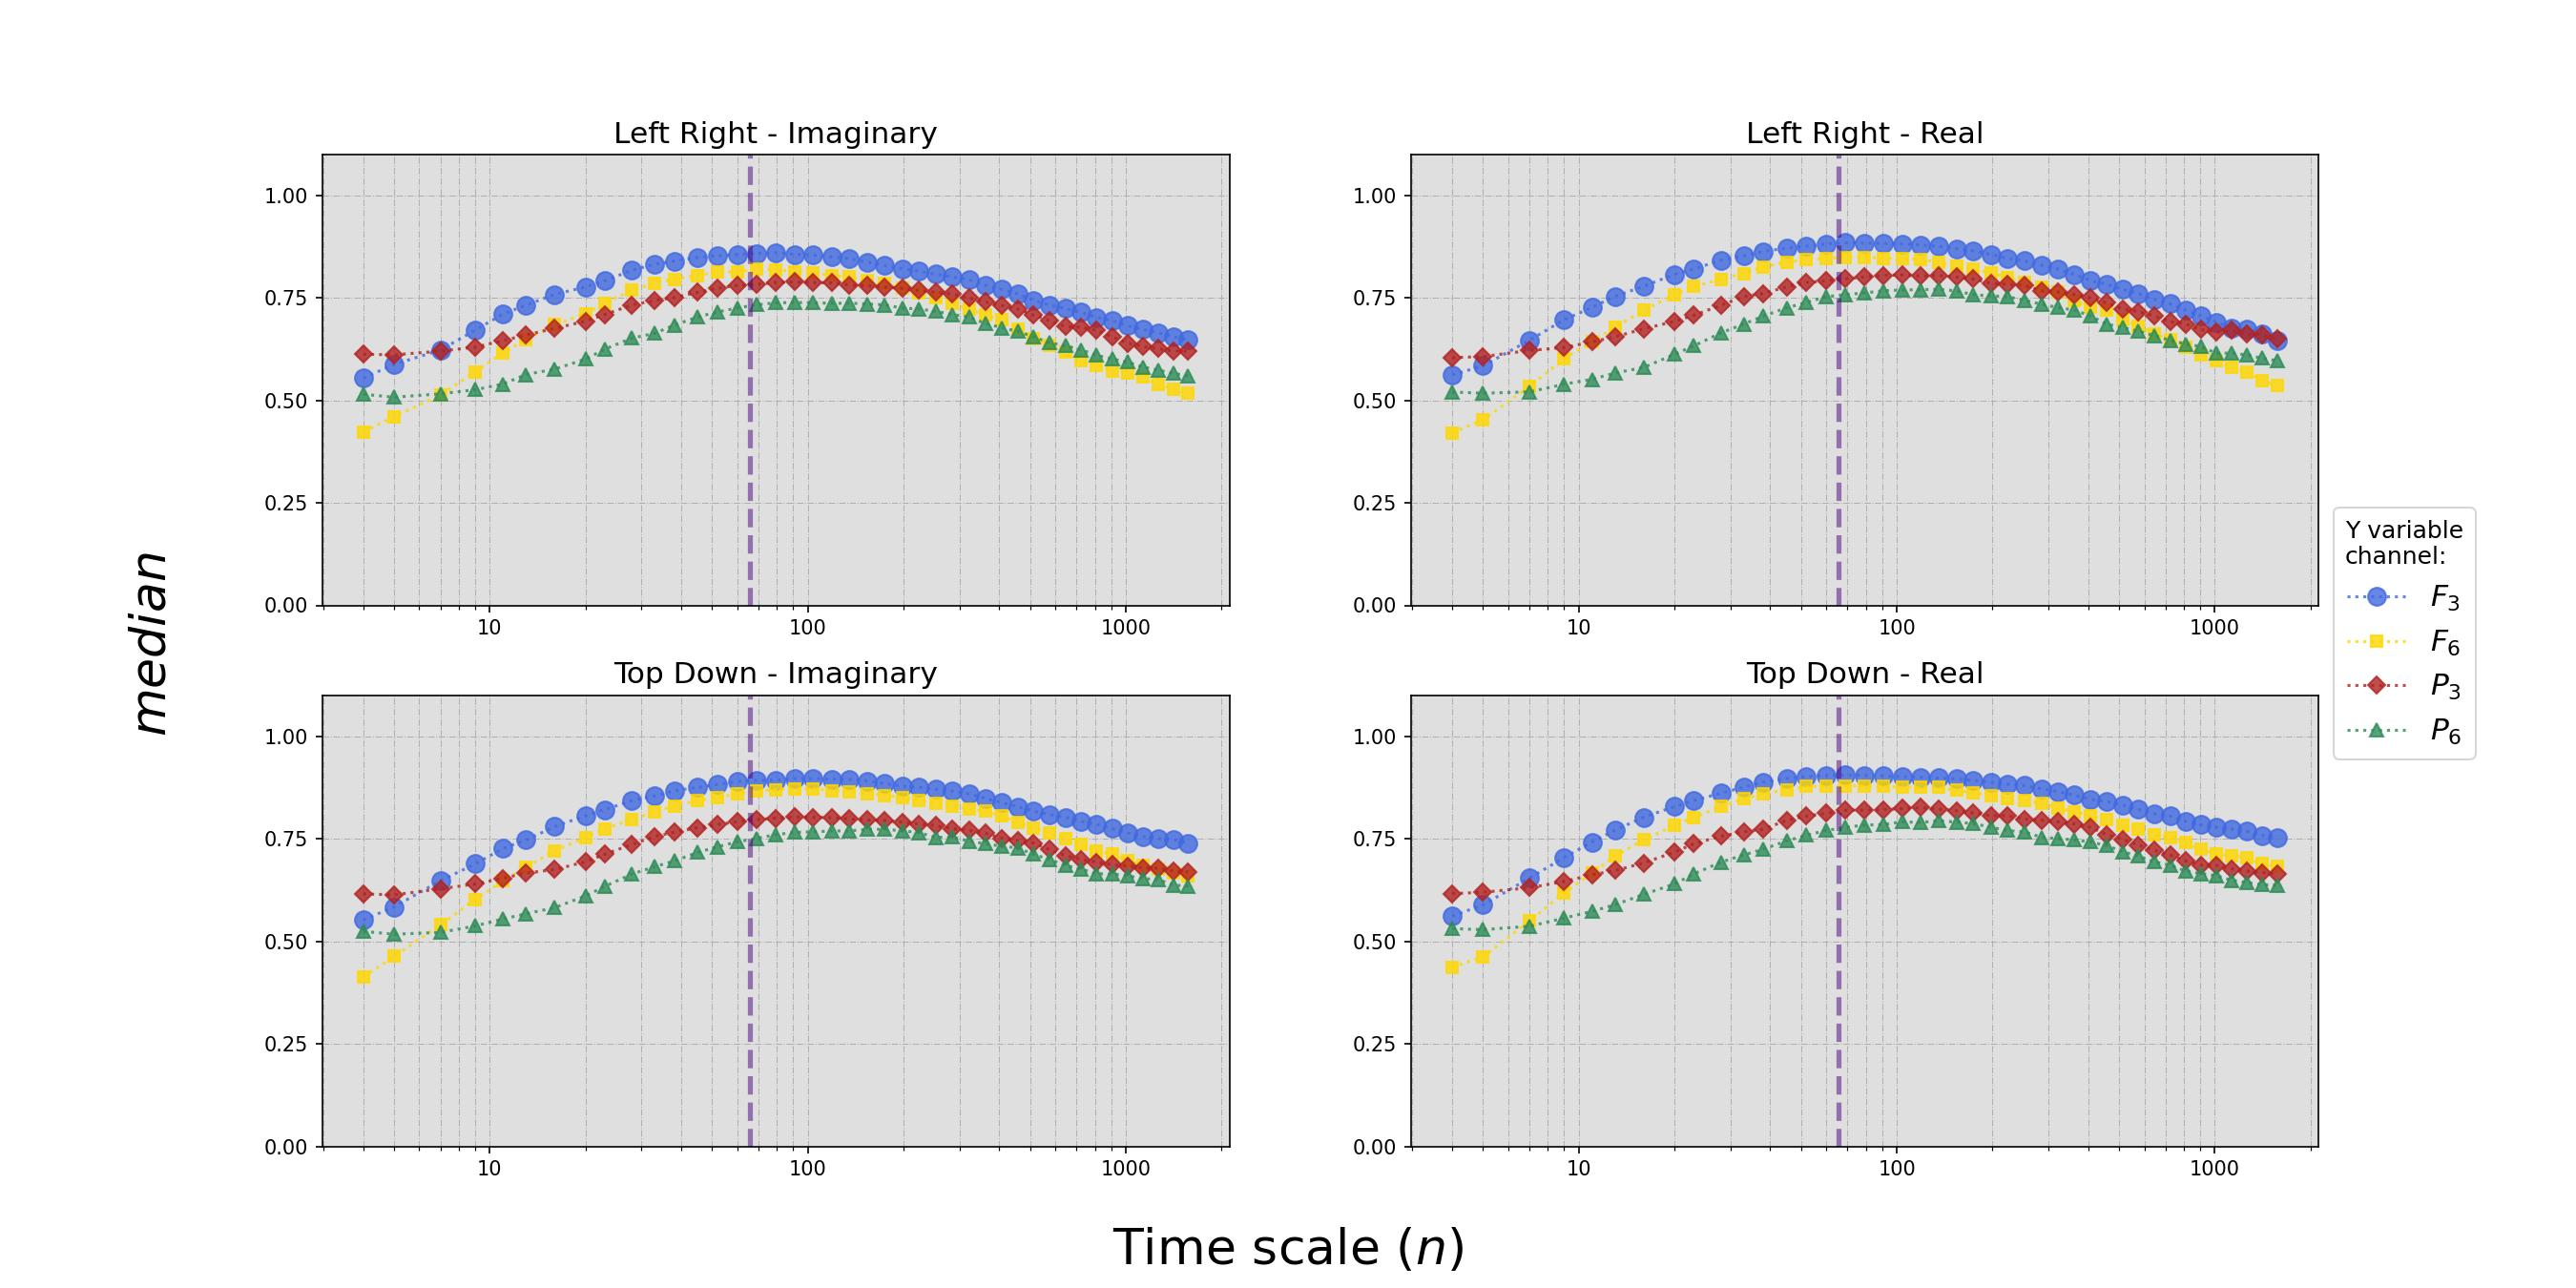
\includegraphics[width=.8\textwidth]{./Figures/art_01/median.jpg}
    \captionsetup{justification=centering}
    \caption{Mediana dos valores do \dmc para cada uma das tarefas.\\  Fonte: Elaborada pelos autores}
	\label{fig:a01_median}
\end{figure}

As Figuras~\ref{fig:a01_sd},~\ref{fig:a01_mean}~e~\ref{fig:a01_median} mostram grande consistência entre a população, no entanto é possível observar características nos gráficos de cada indivíduo que apontam para uma assinatura individual, como uma impressão digital, como explicado no artigo. Para facilitar o entendimento das análises, alguns vídeos que apresentam sequencialmente os resultados das tarefas de cada sujeito foram criados e colocados no repositório \emph{online}.

Nos termos da quantidade de dados analisados, a implementação carece de melhorias e otimizações. Passar os dados para C através da biblioteca \emph{subprocess} é um processo trabalhoso, exigindo a gravação dos arquivos tratados em arquivos formatados conforme as regras estabelecidas no código em C. Generalizações do algorítimo para um número qualquer de séries temporais e do cálculo da inversão da matriz também devem ser implementados para expandir as possibilidades em trabalhos futuros.

\includepdf[pages=-, pagecommand={\thispagestyle{plain}}]{./Papers_publi/Ribeiro_2025_DCCA_multi_cross-correlation_analysis_applied_on_E.pdf}



\section{Artigo 02: A Python/Zig optimized and customizable
implementation for \pdcca~and \dmc~coefficients}
\label{sec:paper_02}

\begin{flushright}
    ``Just remember, once you're over the hill\\
    you begin to pick up speed.''\\[10px]
    (Charles M. Schulz)
    \end{flushright}


O artigo \emph{A Python/Zig optimized and customizable
implementation for \pdcca~and \dmc~coefficients} está sendo revisado com o objetivo de ser publicado na revista \emph{Journal of Statistical Software}. Apresenta um pacote \emph{Python} com métodos de cálculo das funções \dfa~e \dcca e dos coeficientes \pdcca~e \dmc. Os cálculos mais custosos foram implementados em programação de nível mais baixo, utilizando uma linguagem de sistemas, nova e promissora, chamada \emph{Zig}~\url{https://ziglang.org/}. A escolha da linguagem \emph{Zig}~se deu por vários motivos: 

\begin{itemize}
\item Por ser uma linguagem de baixo nível, obtendo velocidades de processamento compatíveis com \emph{C} e \emph{Fortran}~\cite{10820804, Kacs_2024}.
\item Possui compatibilidade com \emph{C} e \emph{C++}, podendo incorporar bibliotecas.
\item Possui uma sintaxe moderna e elegante para tratar problemas de baixo nível.
\item Tem um eficiente sistema de \emph{cross-compilation}.
\end{itemize}

O aspecto das \emph{cross-compilation} foi um dos mais considerados na escolha da linguagem. A manutenção de uma biblioteca por um pequeno grupo de pessoas possui diversos desafios. A capacidade de fornecer programas compilados para diversos sistemas operacionais e arquiteturas de processadores é uma etapa crucial para a popularização de um pacote. A possibilidade de se gerar os executáveis desta biblioteca em um único computador pessoal pareceu uma opção vantajosa.

\begin{algorithm} \caption{Detrended Saved} \label{alg:det_reused}
  \begin{enumerate}[label=4.\alph*]
      \item \textbf{Calculando o \emph{Detrended Value}}: Para cada série $X^{j}$ (incluindo a variável dependente) onde  $1 \ge j \ge m$, sendo $m$ o número de séries temporais; para cada escala temporal, em cada caixa $i$, calcula-se o valor de $DV^{j}_{k,i} = (X^{j}_{k,i}-\widetilde{X^{j}}_{k, i})$ e armazena-se em uma matriz. A matrix tem por dimensões $m, n+1$, onde cada linha corresponde a uma série temporal e as colunas correspondem ao número de pontos em cada caixa.
      \item \textbf{Cálculo da função $f_{DFA}^{2}$ para cada caixa}: Calcula-se o valor do \dfa~:\\[10pt]
          $f_{DFA}^{2}(n, i) = \frac{1}{1+n} \sum_{k=i}^{i + n}(DV^{j1}_{k,i})^{2}$;
      \item \textbf{Cálculo da função $f_{DCCA}^{2}$~em cada caixa}: com a matriz $DV$ devidamente preenchida, para uma das $N - n$ caixas de uma mesma escala temporal a função é calculada para todas as combinações de séries temporais duas à duas por:\\[10pt]
          $f_{DCCA}^{2}(n, i) = \frac{1}{1+n} \sum_{k=i}^{i + n}(DV^{j1}_{k,i}) \times (DV^{j2}_{k,i})$
      \item \textbf{Retomando o algorítimo padrão}: Após o cálculo de todas as caixas, aplica-se o passo 5 do \dfa~e \dcca. 
  \end{enumerate}
  \end{algorithm}

O \emph{software} de cálculo de dinâmica de fluidos computacional \emph{AeroSim}~\url{https://aerosim.io/} apresenta desempenho e precisão nos seus cálculos \cite{romanusViableFrameworkWind2023, lugariniLargeEddySimulations2024} é parcialmente implementado em \emph{Zig} e serviu de incentivo à esta adoção.

Parte da otimização segue a implementação de \citeonline{hartmannRealtimeFractalSignal2013} para o \dfa, transposta para o \dcca~e \pdcca~por~\citeonline{Kapostza2022}. Onde, durante o cálculo da interpolação da reta de tendência, na primeira caixa de cada séries, pelo método dos mínimos quadrados, valores são gravados em variáveis que podem tornar o \emph{loop} de somatórios dos valores utilizados no cálculo dos coeficientes da equação da reta são armazenados em variáveis. Para a caixa seguinte, o \emph{loop} é substituído por operações de subtração e adição.



A Equação~\ref{eq:sum_opt_x}, mostra que o valor da soma das coordenadas no eixo das abscissas de uma caixa pode ser substituído pelo somatório total na caixa anterior menos o primeiro valor de abscissa da caixa anterior, somado ao último valor de $x$ para a caixa atual. Raciocínio análogo pode ser aplicado às Equações~\ref{eq:sum_opt_x2}, \ref{eq:sum_opt_y}~e~\ref{eq:sum_opt_xy}.

\begin{equation}
    \label{eq:sum_opt_x}
    \forall~1<i\leq(N-n),~\sum_{k=i}^{i + n}T_k = \left(\sum_{j=i-1}^{(i+n)-1}T_j\right)~-~T_{i-1}~+~T_{i + n}
  \end{equation}
  
  \begin{equation}
    \label{eq:sum_opt_x2}
    \forall~1<i\leq(N-n),~\sum_{k=i}^{i + n}T_k^2 = \left(\sum_{j=i-1}^{(i+n)-1}T_j^2\right)~-~T_{i-1}^2~+~T_{i + n}^2
  \end{equation}
  
  \begin{equation}
    \label{eq:sum_opt_y}
    \forall~1<i\leq(N-n),~\sum_{k=i}^{i + n}S_k = \left(\sum_{j=i-1}^{(i+n)-1}S_j\right)~-~S_{i-1}~+~S_{i + n}
  \end{equation}
  
  \begin{equation}
    \label{eq:sum_opt_xy}
    \forall~1<i\leq(N-n),~\sum_{k=i}^{i + n} (S_k\times T_k) = \left(\sum_{j=i-1}^{(i+n)-1}(S_j \times T_j)\right)-(S_{i-1} \times T_{i-1})+(S_{i + n} \times T_{i + n})
  \end{equation}

Quando se pensa no cálculo do \dmc, e em como otimiza-lo, deve-se pensar em múltiplos cálculos de \pdcca, para a criação da matriz apresentada na Equação~\ref{eq:p_dcca_matrix}. A ideia é substituir o passo 4 do Algoritmo~\ref{alg:dcca} pelos passos descritos no Algoritmo~\ref{alg:det_reused}.



Essa pequena mudança, embora possa até aumentar o tempo de processamento para um pequeno número de séries temporais, demonstra-se muito vantajoso quanto maior for o número de séries cujo coeficiente \pdcca~ precisa ser calculado.

\begin{equation}\label{eq:combinations_2x2}
  \frac{j!}{2 \times (j-2)!}
\end{equation}

Na biblioteca \emph{Zebende} é possível implementar outras versões do código para o cálculo do \pdcca~com poucas séries temporais. Mas é preciso entender em que ponto o Algoritmo~\ref{alg:det_reused} passa a ser vantajoso.~Caso o $DV$ não seja armazenado, o número de vezes que ele tem que ser calculado é de duas vezes o número de combinações duas a duas para $j$ séries~(Equação~\ref{eq:combinations_2x2}) e o tempo gasto para calcular o $DV$ depende do tamanho das séries.

Vale também ressaltar que as otimizações baseadas no salvamento dos parâmetros do método dos mínimos quadrados pode ser adaptado para diversos graus do polinômio da tendência, mas não pode se adaptar à caixas não sobrepostas.

Como apresentado na Sessão\ref{ss:dfa_fract} do Capítulo~\ref{cap:fund_teorica}, alguns autores ainda advogam pela não sobreposição das caixas~\cite{zhouMultifractalDetrendedCrosscorrelation2008}, nestes casos, o armazenamento dos parâmetros para o cálculo dos mínimos quadrados não funcionaria. Por outro lado, para uma grande quantidade de séries temporais o Algorítimo~\ref{alg:det_reused}, \emph{Detrended Saved}, funcionaria também no cenário de caixas não sobrepostas.

Além da otimização, o artigo apresenta o modo de uso da biblioteca e algumas das funções auxiliares já implementadas. As equações destacadas nas Sessões~\ref{ss:dfa_fract}~e~\ref{ss:vari_cross} do Capítulo~\ref{cap:fund_teorica} estão entre as próximas adições ao pacote.

O código fonte da biblioteca \emph{Zebende} está disponível em \url{https://github.com/255ribeiro/zebende}.


    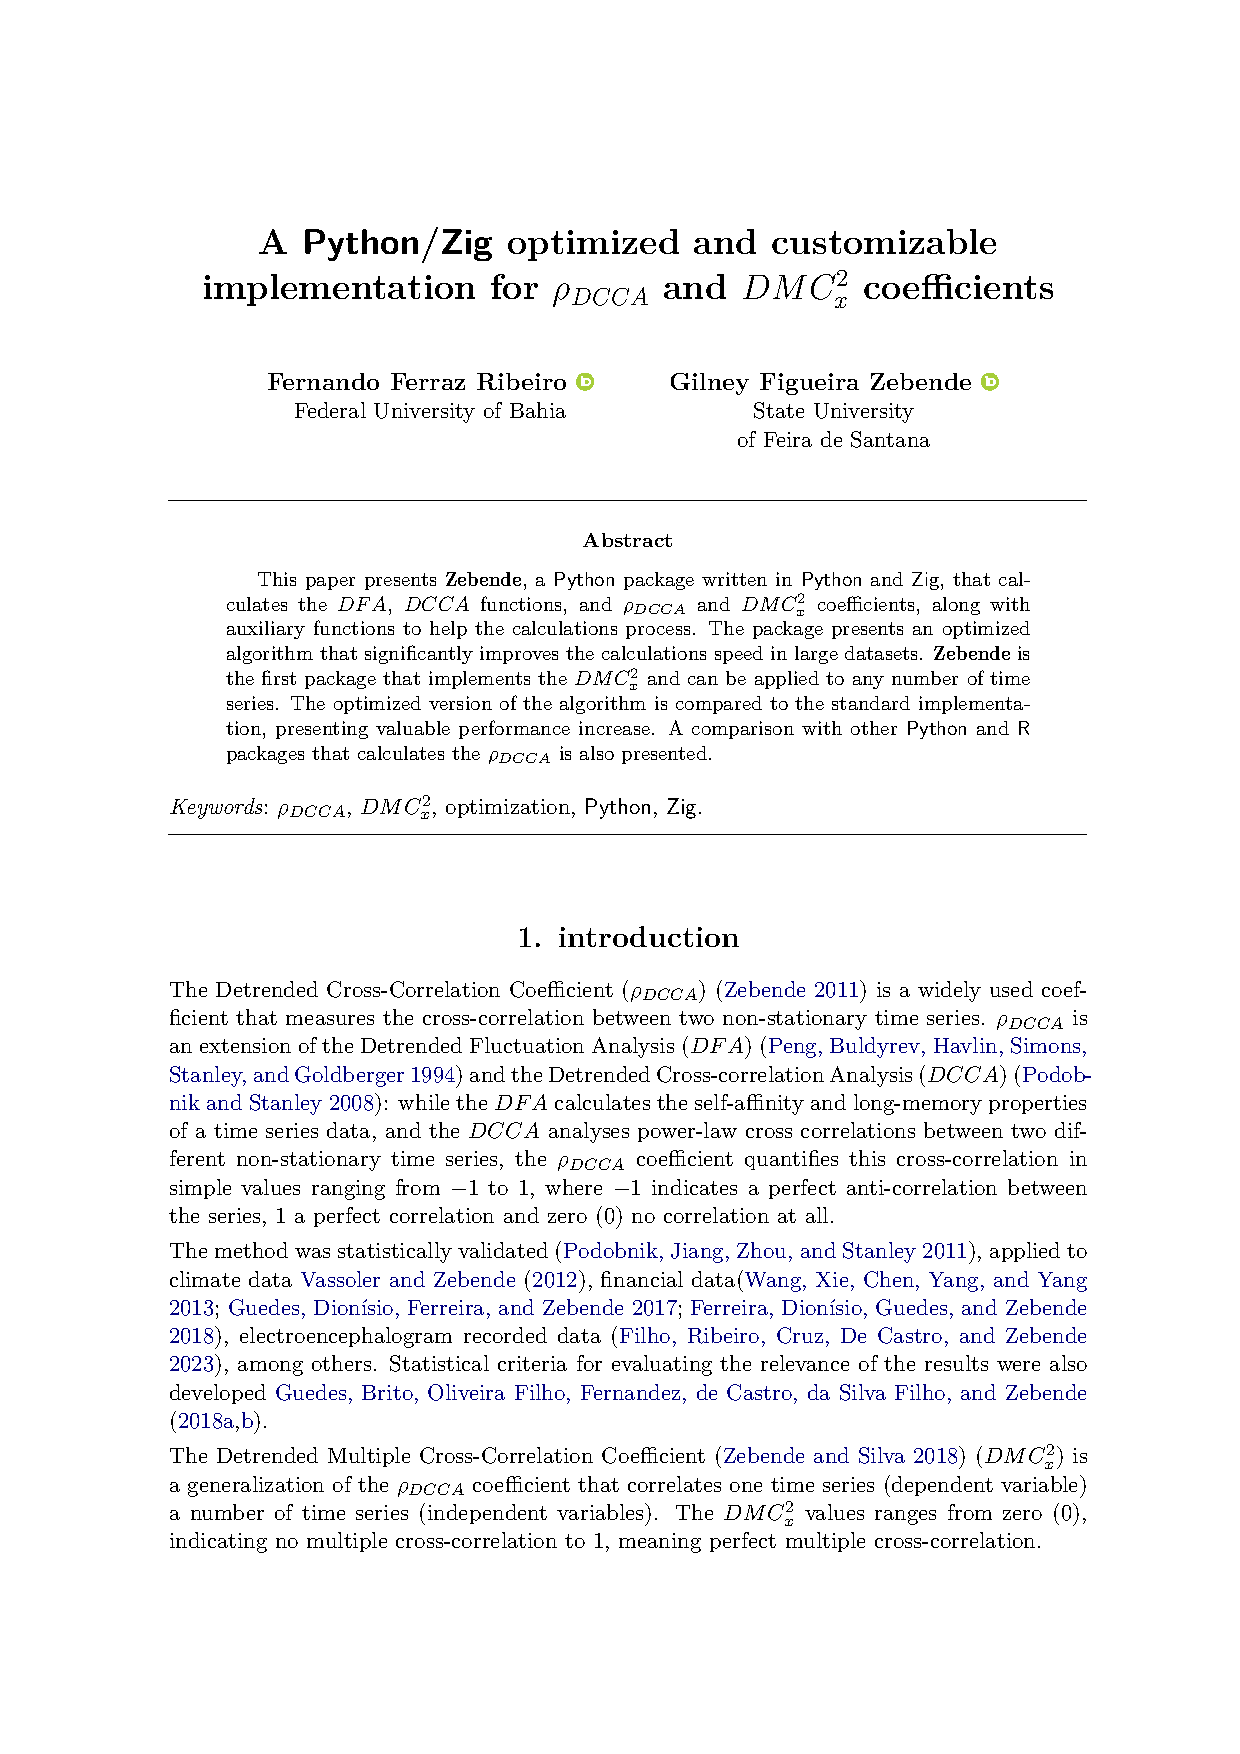
\includepdf[pages=-, pagecommand={\thispagestyle{plain}}]{./Papers_publi/paper_zebendelib.pdf}

% ----------------------------------------------
% ------------------------------------------

\section{Maximização do coeficiente \dmc utilizando matriz \pdcca~e $DPDCCA$}\label{sec:paper_03}



\begin{flushright}
    ``Noel Meyerhof consulted the list he had prepared \\
    and chose which item was to be first. \\
    As usual, he relied mainly on intuition.''\\[10px]
    (Isaac Asimov)
    % Isaac Asimov - Jokester - 1956
    \end{flushright}

\begin{figure}[!htb]
	\centering
	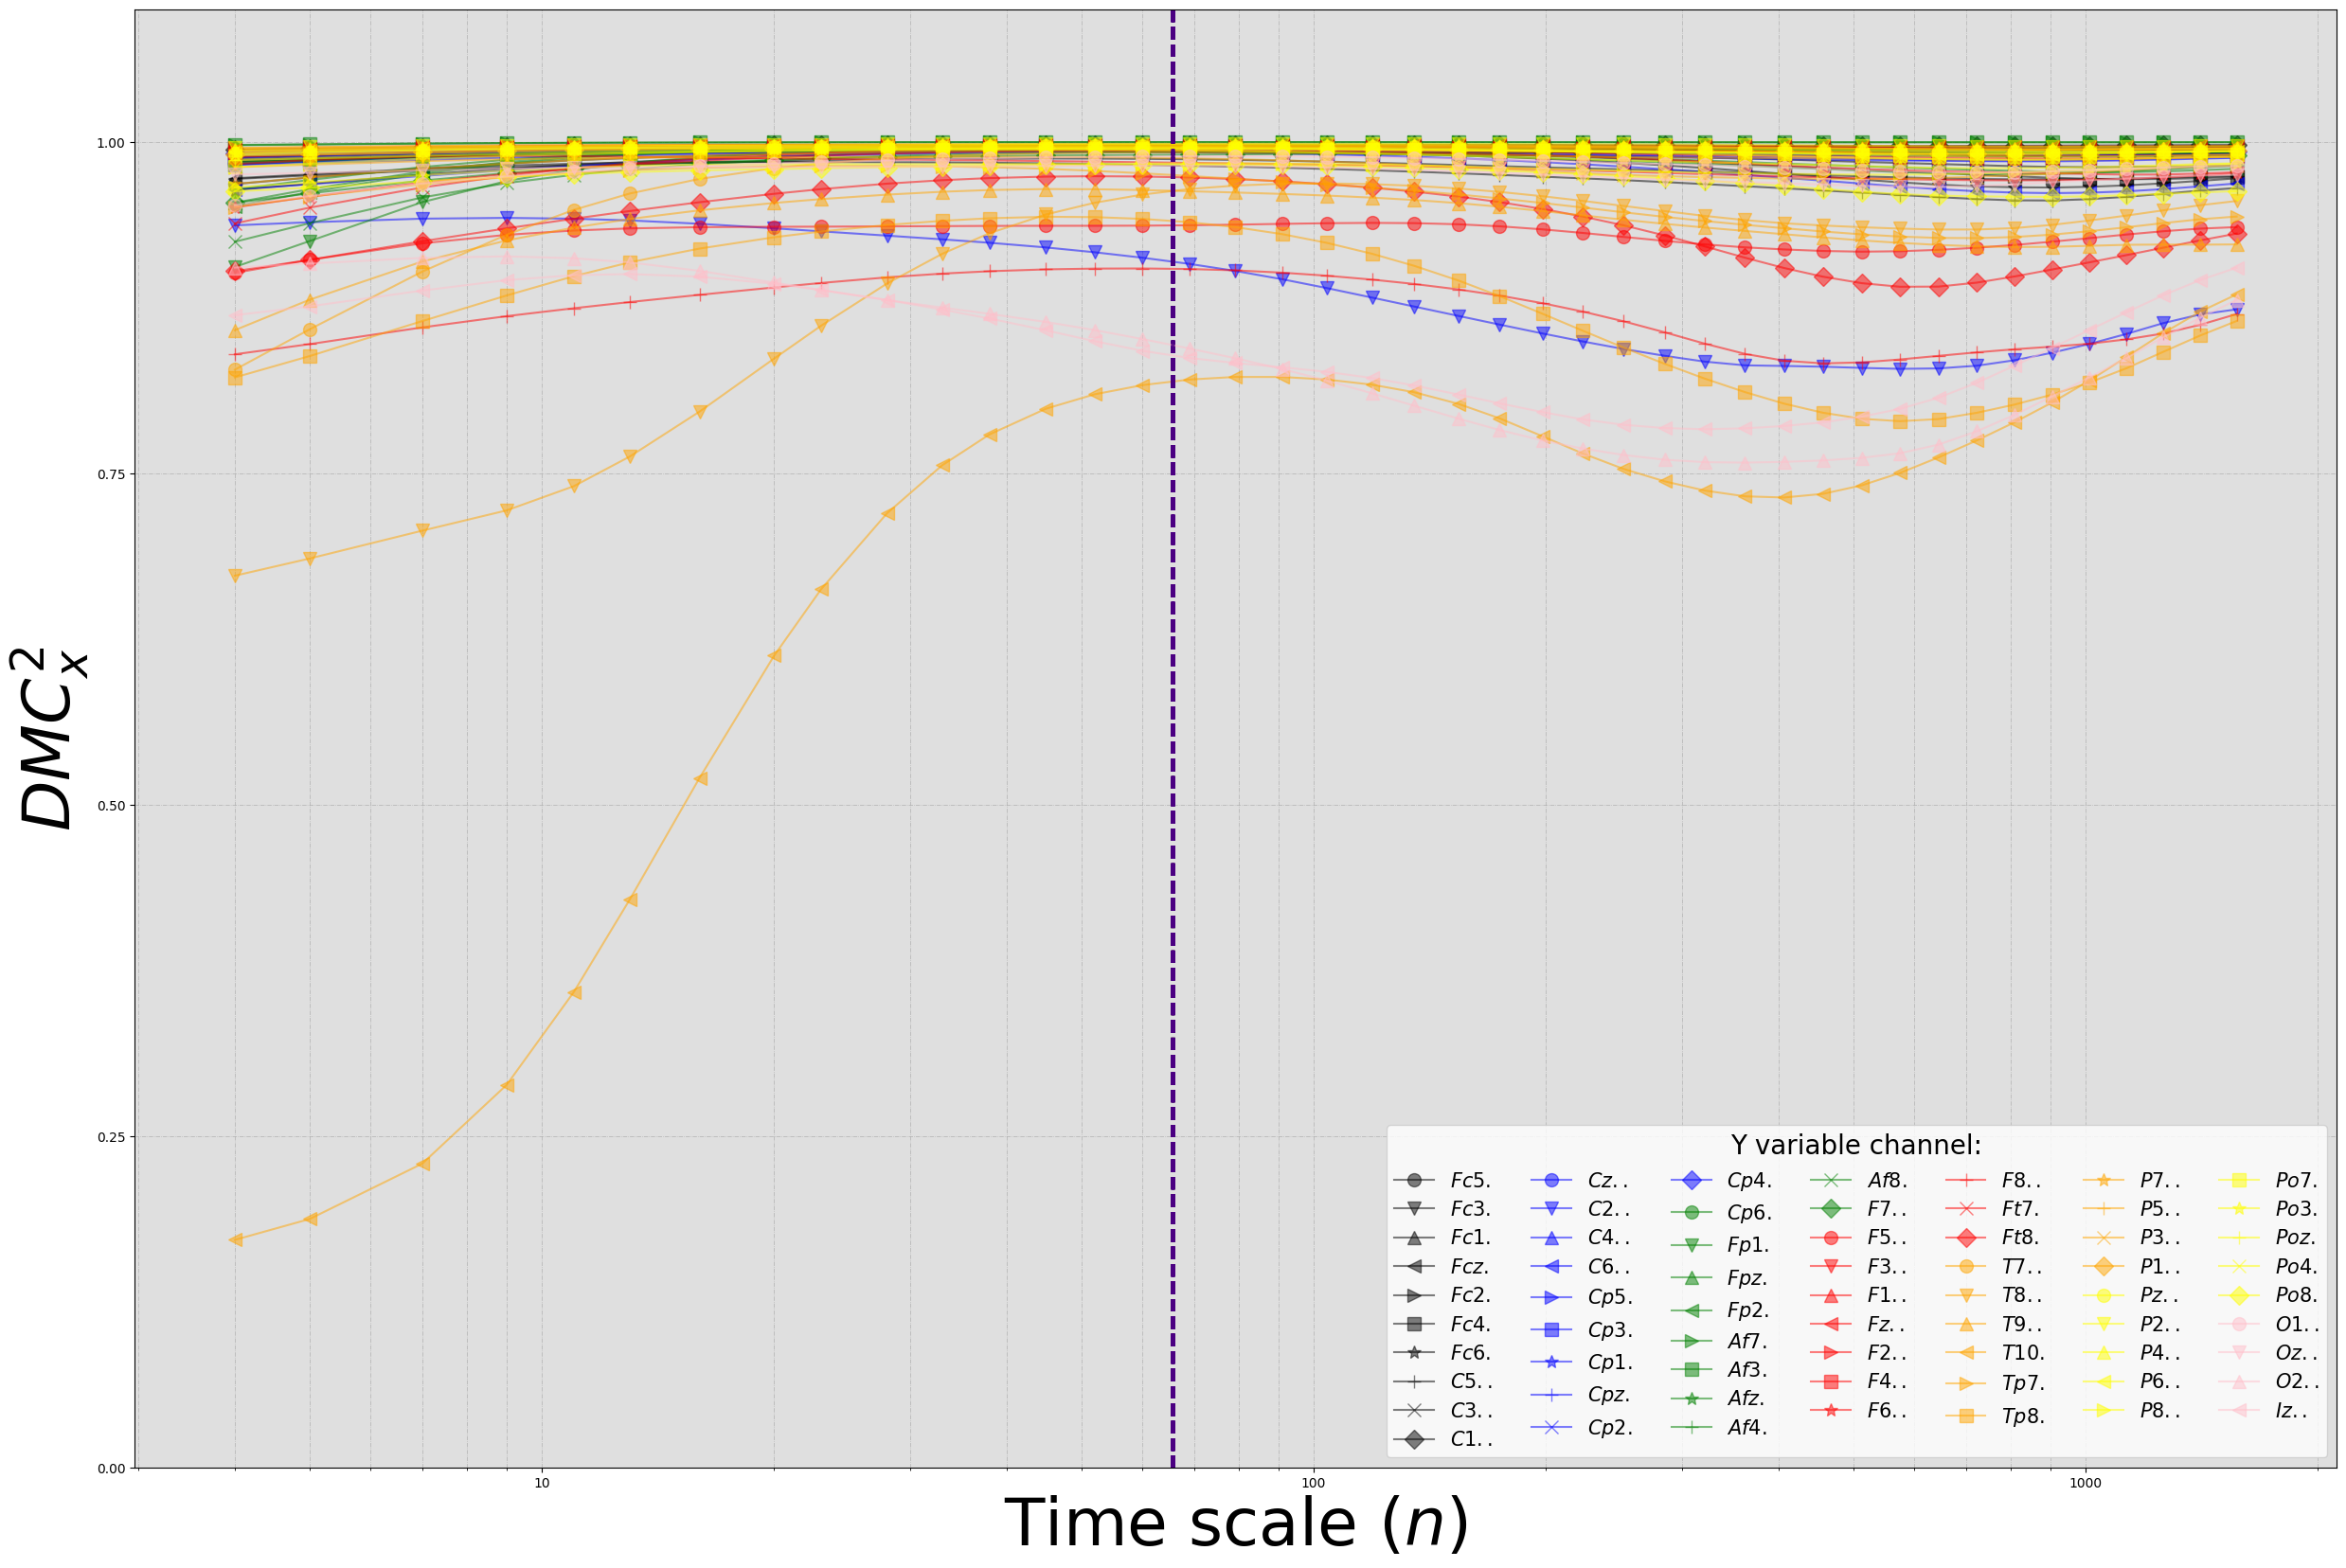
\includegraphics[width=.95\textwidth]{./Figures/art_03/dmc_all.png}
  \captionsetup{justification=centering}
  \caption{\dmc~de todo os canais do experimento[1:63] para cada canal como variável dependente.\\Fonte: Elaborada pelos autores}

	\label{fig:a03_dmc_total}
\end{figure}

Com a ferramenta desenvolvida e testada, volta-se para os dados utilizados nos artigos do Capítulo~\ref{cap:cap3} Sessão~\ref{sec:paper_01}, e no Anexo~\ref{an:a}. A matriz do \pdcca~para todos os $64$ canais é calculada em menos de $17min$. Isso se deve ao Algoritmo \emph{Detrended Saved}. Sem a aplicação deste, calculando o número de combinações necessárias para a montagem da matriz (Equação~\ref{eq:combinations_2x2}), levando em conta que, para cada \dcca~aplica-se duas vezes o cálculo do $DV$, chega-se ao valor de $2016 \times 2 = 4032$. Com o uso do algoritmo, apenas $64$ valores são calculados.

Com a matriz montada, o cálculo do \dmc, envolvendo todas as $64$ séries, com cada uma delas como variável dependente, para os $42$ valores de $n$, utilizados nos referidos artigos, é realizado em $0.7s$.

A Figura~\ref{fig:a03_dmc_total} apresenta esses resultados. Apontando para um sistema altamente correlacionado. Também encontramos um pico de correlação entre as escalas $n=60$ e $n=69$, confirmando o encontrado nos artigos.

A inversa de cada uma das $42$ matrizes do \pdcca~também foi calculada em menos de $1s$. O $DPDCCA$ foi implementado e calculado para todas as combinações de canais, para cada escala temporal, levando também menos de $1s$ na execução.

É evidente o aumento na quantidade de informações que se pode obter e tratar com as ferramentas computacionais desenvolvidas neste trabalho. É necessário desenvolver instrumentos para acessar essas informações.



 

\subsection{Metodologia}

Um experimento foi montado, investigando o quanto partindo da premissa:

\begin{itemize}
  \item Nem todos os canais contribuem igualmente para o \dmc~de uma série como variável dependente e todas as outras como dependente;

\end{itemize}

foram elaboradas a hipótese:

\begin{itemize}
  \item é possível selecionar um subconjunto pequeno de canais cujo \dmc~se aproxime do valor total.
\end{itemize}

Para testar a hipótese, foi escolhido o canal \emph{T8}. Em um sistema tão correlacionado, um canal que, para $n=4$ afasta-se muito do conjunto mais correlacionado e, no pico de multi-correlação mostrado na Figura~\ref{fig:a03_dmc_total}, aproxima-se do citado conjunto, aparenta-se como um candidato interessante para as primeiras avaliações.

Optou-se pela escolha do \dmc de $1:8$ canais, representando $1/8$ do total de canais, para comparar com o valor do \dmc$1:64$. As escalas temporais $n=4$ e $n=69$ foram escolhidas.

Foram estabelecidos cinco modelos para escolher os 8 canais que mais contribuem para o \dmc~total:

\begin{itemize}
  \item Aleatório: como um artifício de controle.
  \item \pdcca : Os oito maiores valores do \pdcca de \emph{T8} em relação À cada uma das outras variáveis.
  \item $|$\pdcca$|$ : Os oito maiores valores absolutos do \pdcca de \emph{T8} em relação À cada uma das outras variáveis.
  \item $DPDCCA$ : Os oito maiores valores do $DPDCCA$ de \emph{T8} em relação À cada uma das outras variáveis.
  \item $\Sigma DPDCCA$ : Um algoritmo baseado nas características do $DPDCCA$.  
\end{itemize}


\begin{algorithm} \caption{$\Sigma DPDCCA$} \label{alg:edpdcca}
  \begin{lstlisting}
  def maximize_dmc_dp(n, index, count, c_mat ):
    dmc_of = [index]
    for i in range(count):
        comp_array = np.full(64, fill_value = np.nan, dtype = float)
        for j in range(64):
            if j in dmc_of:
                pass
            else:
                for k in dmc_of:
                    temp = pddcca(j, k, n, c_mat)
                    if  np.isnan(comp_array[j]):
                        comp_array[j] = temp
                    else:
                        comp_array[j] += temp
        dmc_of.append(int(np.nanargmax(comp_array)))
    return np.array(dmc_of)

    \end{lstlisting}
\end{algorithm}

O critério de seleção $\Sigma DPDCCA$ aparece está apresentado, em código, no Algoritmo~\ref{alg:edpdcca}. O $DPDCCA$ tem características particulares. Analisando a Equação~\ref{eq:dpdcca} ve-se que, entre duas séries idênticas, obtêm-se o valor mais baixo possível $-1$, indicando que a informação daquela série não agrega valor ao todo.

Pelo critério do $\Sigma DPDCCA$, a escolha dos 8 canais acontece de forma sucessiva. O primeiro canal é escolhido pelo maior valor do $DPDCCA$ em relação ao canal \emph{T8}. Para os próximos $7$ canais, calcula-se o maior valor do $DPDCCA$ entre o canal candidato e o canal \emph{T8} somado com os valores de $DPDCCA$ entre o canal candidato e os canais escolhidos nas etapas anteriores.


\subsection{Resultados}

A Tabela~\ref{tab:time_4} apresenta os resultados dos cinco métodos para $n=4$. O valor de referência é o valor do \dmc~de \emph{T8} com todos os outros canais. Os métodos aparecem na primeira coluna, Os canais selecionados na segunda, o valor do \dmc~de \emph{T8} em relação aos canais selecionados na terceira e o percentual do valor obtido em relação ao valor de referência na última coluna.

\begin{table}[h!]
    \centering
    \caption{Maximização do \dmc. $n=4,~ count=8$, referência$= 0.6726$} \label{tab:time_4}
    \begin{tabular}{c|c|c|c}
      \hline
      Critério & canais selecionados & valor & percentual \\
      \hline
      \hline
      \pdcca & T8 Fc6 C6 Cp6 F6 F8 Ft8 P4 P6 & 0.6330  & 94.1108\% \\
      $|$ \pdcca $|$ & T8 Fc6 C6 Cp6 F6 F8 Ft8 P4 P6  & 0.6330 & 94.1108\% \\
      $\Sigma DPDCCA$ & T8 Fc6 C6 Cp6 F2 F4 F6 F8 Ft8 & 0.6329 &  94.0908\% \\
      $DPDCCA$ & T8 C6 Cp6 Fp2 Afz F3 F4 Ft8 P6 & 0.5686 & 84.5341\% \\
      Random & T8 P6 P5 C1 F1 F4 Cp6 Fc1 F6 & 0.3138 & 46.6517\% \\
      
      \hline
    \end{tabular}
  \end{table}

  Os valores do \pdcca, do $|$ \pdcca $|$~ e do $\Sigma DPDCCA$ aproximam em tono de $94.1\%$, com o \pdcca, e o $|$ \pdcca $|$~escolhendo os mesmos canais e performando levemente acima do $\Sigma DPDCCA$, que escolheu os canais \emph{F2} e \emph{F8} em vez dos canais \emph{P4} e \emph{P6}. O desempenho do critério $DPDCCA$ fica abaixo dos já citados.

  \begin{table}[h!]
    \centering
    \caption{Maximização do \dmc. $n=69,~ count=8$, referência$=0.9643 $} \label{tab:time_69}
    \begin{tabular}{c|c|c|c}
      \hline
      Critério & canais selecionados & valor & percentual \\
      \hline
      \hline
      \pdcca & T8 Fc4 Fc6 C4 C6 Cp6 F6 Ft8 Tp8 & 0.9581  & 99.3548\% \\
      $|$ \pdcca $|$ & T8 Fc4 Fc6 C4 C6 Cp6 F6 Ft8 Tp8  & 0.9581 & 99.3548\% \\
      $\Sigma DPDCCA$ & T8 Fc6 C6 Cp6 Ft8 T10 Tp8 P6 P8 & 0.9597 &  99.5189\% \\
      $DPDCCA$ & T8 C6 Cp6 Ft8 T7 T10 Tp7 Tp8 P8 & 0.9572 & 99.2568\% \\
      Random & T8 Fp1 Po7 F7 P6 Cp3 C3 Po4 P2 & 0.8083 & 83.8165\% \\
      \hline
    \end{tabular}
  \end{table}

  Na tabela~\ref{tab:time_69} ve-se resultados semelhantes. Nesta escala temporal com maior multi-correlação, aparece o $\Sigma DPDCCA$ um pouco acima dos outros e com o critério $DPDCCA$ mais próximos dos demais. Diferenças entre os canais escolhidos em uma escala temporal para a outra também foram registrados.

  A semelhança entre os critérios \pdcca~e $|$ \pdcca $|$~ se deve à característica do sistema de além de ser fortemente muli-correlacionado, também é positivamente multi-correlacionado. Desconsiderando o \pdcca~de um canal com ele mesmo, os valores de \pdcca~variam de $0.9995$ até o mínimo de $-0.2281$. Não existem anti-correlações significativas em nenhuma das escalas temporais calculadas. 

\subsection{Conclusão}

Os critérios $|$ \pdcca $|$~e $\Sigma DPDCCA$~apresentaram bons resultados na maximização do coeficiente \dmc em relação ao total. É recomendado a repetição do experimento em mais escalas temporais e com outros canais como variável dependente.

Os critérios de aproximação também podem ser entendidos como critérios de semelhança entre séries. Se bem entendidos e validados por extensões desta pesquisa.

A ideia de maximizar o coeficiente apresenta similaridades com o processo de seleção de atributos em um algoritmo de aprendizado de máquina. Os resultados preliminares podem ser entendidos como um indício de que o desempenho destes critérios para a seleção de atributos devem ser verificados.